% 图 1.7 外磁场中经典电子体系的回旋轨道：体内轨道相互抵消，边界形成净环流
\documentclass[tikz,border=5pt]{standalone}
\usetikzlibrary{arrows.meta,decorations.markings}
\usepackage{amsmath}
\usepackage{bm}
\usepackage{fontspec}
\setmainfont{Times New Roman}
\begin{document}
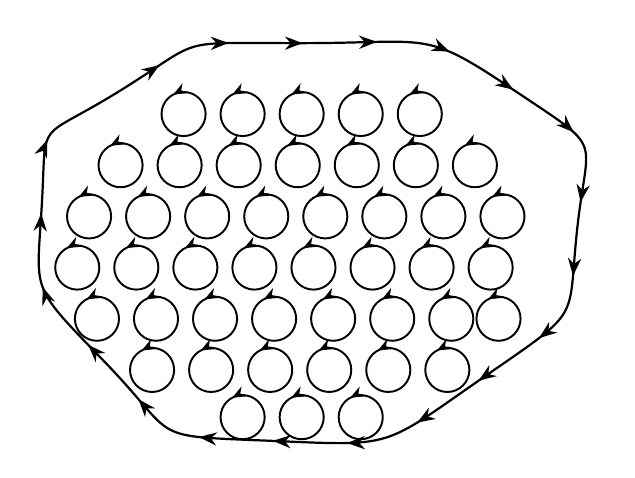
\begin{tikzpicture}[line width=0.8pt,>=Stealth]
% 样品边界（沿边界顺时针的小箭头：表面净环流方向）
\draw[postaction={decorate,decoration={markings,
  mark=between positions 0.03 and 0.96 step 0.048 with
    {\arrow[line width=0.75pt]{Stealth}}}}]
  plot[smooth cycle,tension=1.2] coordinates
  {(-3.3,0.5) (-2.3,1.95) (0,2.55) (2.7,1.95) (3.5,0.2)
   (2.3,-1.7) (-0.4,-2.5) (-2.5,-1.5)};
% 体内回旋轨道（逆时针小环）
\foreach \px/\py in {-1.5/1.65,-0.75/1.65,0/1.65,0.75/1.65,1.5/1.65,
 -2.3/1.0,-1.55/1.0,-0.8/1.0,-0.05/1.0,0.7/1.0,1.45/1.0,2.2/1.0,
 -2.7/0.35,-1.95/0.35,-1.2/0.35,-0.45/0.35,0.3/0.35,1.05/0.35,1.8/0.35,2.55/0.35,
 -2.85/-0.3,-2.1/-0.3,-1.35/-0.3,-0.6/-0.3,0.15/-0.3,0.9/-0.3,1.65/-0.3,2.4/-0.3,
 -2.6/-0.95,-1.85/-0.95,-1.1/-0.95,-0.35/-0.95,0.4/-0.95,1.15/-0.95,1.9/-0.95,2.5/-0.95,
 -1.9/-1.6,-1.15/-1.6,-0.4/-1.6,0.35/-1.6,1.1/-1.6,1.85/-1.6,
 -0.75/-2.2,0/-2.2,0.75/-2.2}{
  \draw[line width=0.7pt] (\px,\py) circle (0.28);
  % 逆时针箭头（圆顶部，指向左）
  \draw[line width=0.7pt,-{Stealth[length=1.7mm,width=1.4mm]}]
    (\px,\py) ++(85:0.28) arc[start angle=85,end angle=118,radius=0.28];
}
\end{tikzpicture}
\end{document}
